\newpage

% Из текста короткого задания на ВКР:
% 1. Проанализировать технологии, используемые для реализации бесконтактного взаимодействия платежного терминала и средства платежа (карты, смартфона и пр.).
% 2. Проанализировать методы и инструменты обеспечения безопасности бесконтактных платежей
% -. Сравнение существующих аналогов систем коррекции
% -. Выбор методы и технологий разработки системы


%  - Как технически выглядит процесс оплаты (от введения суммы и прикладывания карты, до отображения статуса платежа)
%  - Декомпозиция процесса на технологии, используемые на разных этапах
%  - Обзор технологий
%    - с точки зрения тех. процесса
%    - с точки зрения безопасности
%  - Сравнительный анализ существующих решений
%  - Формирование требований к системе (используемые технологии, превосходство над аналогами)

\section{Анализ предметной области}

\subsection{Развитие сферы банковских платежей}

\subsubsection{Эволюция платежных операций}

Появление банковской системы, выступающей в качестве посредника между государством и гражданами, ознаменовало процесс непрерывного развития финансовых технологий, поскольку банки стремились повысить свою прибыльность, в том числе путем повышения качества платежных сервисов.
Деньги выступали в качестве основного способа оплаты товаров и услуг, однако не всегда были удобным способом оплаты, поэтому в дополнение к ним сначала появились бумажные чеки, а позднее и банковские карты.
Вместе с появлением банковских карт, появились и платежные системы~-- инстанции, которые не только выпускали и поддерживали карты, но и выступали посредниками между банками.
Для приема карт к оплате необходимы были специальные устройства.
Изначально это были импринтер, с помощью которого создавались слипы~-- бумаги, содержащие реквизиты карты, дату и сумму покупки и др..
Ему на смену пришел электронный терминал оплаты (POS-терминал), который упрощал взаимодействие с картой, т.к. передавал информацию о карте напрямую в процессиноговые центры платежной системы.

При приеме карты кассир должен был получить информацию от банка, что у держателя карты есть необходимый объем денежных средств для оплаты, в противном случае товар или услуга не могла быть оплачена.
Изначально этот процесс выглядел следующим образом: кассир звонил в банк-эквайер, тот связывался с банком-эмитентом, выпустившем карту, который подтверждал наличие необходимой суммы и инициировал ее передачу в банк-эквайер либо сообщал о невозможности оплаты.
Платежные системы изначально выступали каналом связи между банками.
Однако с увеличением количества карт создавалась высокая нагрузка на банки, и с целью ее снижения появились специальные процессинговые центры, которые совместно с платежными системами осуществляли функцию клиринга~\cite{habr_fondy_payment_history}.

Клиринг~-- это комплекс взаиморасчётов за оказанные услуги, проданные товары или ценные бумаги, основанные на безналичных расчётах.
Клиринг в платёжной системе~-- это взаиморасчёты по любым операциям, совершённым с помощью банковской карты.
Функцию клиринга выполняет ПС, за счет нее снижается нагрузка на банки, выступающие в роли эквайеров, т.к. ПС переводит им деньги в конце операционного дня~\cite{habr_nspk_cliring}.

Процесс идентификации голосом постепенно ускорялся, за счет повышения стабильности и качества телефонии.
Однако с ужесточением требованием ПС к времени подтверждения транзакции и развития банковских алгоритмов ему на смену пришла авторизация по пин-коду, которая является актуальной технологией на данный момент.
ПС совместно с банками продолжают развивать технологию авторизации, в результате чего сейчас для выполнения платежных операций, не превышающих определенный лимит, не требуется пин-код.

Также на текущий момент в России активно развивается оплата посредством QR-кодов, предоставляемых Системой Быстрых Платежей (СБП) и/или банками-эквайерами.
Данная технология не новая, однако оказалась востребованной среди пользователей, поскольку для оплаты по QR подойдет любое мобильное устройство с камерой и выходом в интернет. 
А после наложения на Россию санкций в 2022-м году смартфоны под управлением ОС IOS лишились возможности оплаты посредством NFC, и оплата по QR-коду стала единственно-возможным вариантом~\cite{habr_nspk_qr}.


\subsubsection{Эволюция банковских карт}

Банковские карты так же, как и сами платежные операции, претерпели ряд изменений.
Сначала в них появилась магнитная полоса для быстрой идентификации карты платежным терминалам с помощью статических данных, хранимых в карте.
В 1993 году международные платёжные системы Mastercard, Visa и Europay подписали соглашение о совместной работе, чтобы развить технологии банковских карт.
В результате чего в 1994 году была выпущена первая версия стандарта EMV и систем на его основе.

Данный стандарт предусматривал наличие специального EMV-чипа, встроенного в карты.
Данный чип~-— это микропроцессор, предназначенный для безопасного хранения и обработки данных при проведении платежных операций.
В отличие от традиционной магнитной полосы, которая содержит статичные данные и легко подделывается, EMV-чип генерирует уникальный криптографический код для каждой транзакции, что делает её практически невозможной для подделки~\cite{emv_specifications_book}.

EMV-стандарт был внедрен с целью глобального повышения безопасности безналичных платежей и снижения уровня подделки карт и кражи их данных.
EMV-стандарт ввел понятие офлайн транзакции~-- платежной операции исключительно с участием карты и платежного терминала, которые проводит ее аутентификацию.
В онлайн транзакции терминал связывается в режиме реального времени с банком-эквайером, который через ПС запрашивает аутентификацию карту у банка-эмитента.

После массового внедрения EMV-карт во многих странах наблюдалось значительное снижение случаев фрода с использованием поддельных карт~\cite{plas_emv_fraud}.
Фрод~-- это проведение мошеннических (неправомерных) операций с использованием банковских карт.
Кроме того, EMV-чип лег в основу технологий бесконтактной оплаты, таких как PayPass (Mastercard), payWave (Visa) и Mir Accept (НСПК), где также используется принцип одноразовых криптограмм.
Бесконтактные карты используют технологию радичастотной модуляции сигнала (RFID), с использованием антенны, встроенной в карту, представленной на рисунке~\ref{fig:emv_card}.

\begin{figure}[H]
    \centering
    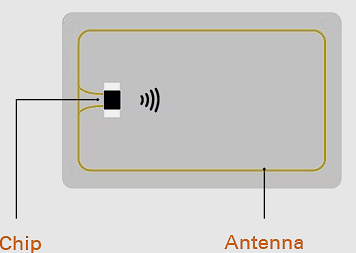
\includegraphics[width=0.4\textwidth]{images/research/emv_card}
    \caption{\centering Структура бесконтактной EMV-карты}
    \label{fig:emv_card}
\end{figure}

С распространением технологии NFC появилась сфера мобильных платежей.
Покупатели получили возможность быстро и безопасно выполнять оплату посредством устройств с поддержкой NFC с помощью виртуальных карт, добавленных в приложение «цифрового кошелька».
Примеры подобных приложений: Apple Pay, Google Pay, Mir Pay и др..


\subsection{Анализ процесса платежа через терминал}



\subsection{Анализ платежных технологий}



\subsection{Сравнительный анализ существующих решений}


\subsection{Формирование требований к системе}


